\documentclass[11pt]{article}

\usepackage[portuguese]{babel}
\usepackage[utf8]{inputenc}
\usepackage{amsmath}
\usepackage{graphicx}
\usepackage{float}
\usepackage{subfig}
\usepackage{fixltx2e}
\usepackage[bottom]{footmisc}
\usepackage{listings}
\usepackage{color} 
\usepackage[usenames,dvipsnames]{xcolor}
\usepackage[colorinlistoftodos]{todonotes}
\usepackage[font=footnotesize]{caption}

\definecolor{keywordcolor}{rgb}{0,0.4,0.7}
\definecolor{commentcolor}{rgb}{0.4,0.4,0.4} 	
\definecolor{mygray}{rgb}{0.5,0.5,0.5} 	% line counter color
\definecolor{mymauve}{rgb}{0.90,0.25,0.47}	% string color
\definecolor{codebackground}{rgb}{0.95,0.95,0.95} 

\lstset{ %
	backgroundcolor=\color{codebackground},   % choose the background color; you must add \usepackage{color} or \usepackage{xcolor}
	basicstyle=\ttfamily \footnotesize,        % the size of the fonts that are used for the code
	breakatwhitespace=false,         % sets if automatic breaks should only happen at whitespace
	breaklines=true,                 % sets automatic line breaking
	captionpos=b,                    % sets the caption-position to bottom
	commentstyle=\color{commentcolor},    % comment style
	deletekeywords={...},            % if you want to delete keywords from the given language
	escapeinside={\%*}{*)},          % if you want to add LaTeX within your code
	extendedchars=true,              % lets you use non-ASCII characters; for 8-bits encodings only, does not work with UTF-8
	keepspaces=true,                 % keeps spaces in text, useful for keeping indentation of code (possibly needs columns=flexible)
	keywordstyle=\color{keywordcolor},       % keyword style
	numbers=left,                    % where to put the line-numbers; possible values are (none, left, right)
	numbersep=5pt,                   % how far the line-numbers are from the code
	numberstyle=\tiny\color{mygray}, % the style that is used for the line-numbers
	rulecolor=\color{black},         % if not set, the frame-color may be changed on line-breaks within not-black text (e.g. comments (green here))
	showspaces=false,                % show spaces everywhere adding particular underscores; it overrides 'showstringspaces'
	showstringspaces=false,          % underline spaces within strings only
	showtabs=false,                  % show tabs within strings adding particular underscores
	stepnumber=1,                    % the step between two line-numbers. If it's 1, each line will be numbered
	%stringstyle=\color{mymauve},     % string literal style
	  identifierstyle=\color{mymauve},
	tabsize=2                       % sets default tabsize to 2 spaces
}

\setcounter{tocdepth}{1}

\numberwithin{equation}{section}

\linespread{1.3}
\usepackage{indentfirst}
\usepackage[top=2cm, bottom=2cm, right=2.3cm, left=2.3cm]{geometry}
\addto\captionsportuguese{\renewcommand{\contentsname}{Índice}}

\begin{document}

\begin{titlepage}
\begin{center}

\hfill \break
\hfill \break


\includegraphics[width=0.3\textwidth]{./logo}~\\[1cm] 

\textsc{\LARGE Instituto Superior Técnico}\\[0.25cm]
\textsc{\Large Mestrado Integrado em Engenharia Electrotécnica e de Computadores}\\[1.8cm]
\textsc{\huge Sistemas Electrónicos de Processamento de Sinal}\\[0.25cm]

\vspace{6mm}

{\huge \bfseries NCO \linebreak \& \linebreak Transmissor BPSK \\[1cm]}

\begin{tabular}{ l l }
Maria Margarida Dias dos Reis & \hspace{2mm} n.º 73099 \\
David Gonçalo C. C. de Deus Oliveira & \hspace{2mm} n.º 73722 \\
Nuno Miguel Rodrigues Machado & \hspace{2mm} n.º 74236
\end{tabular}

\vspace{7mm}

Grupo n.º 5 de segunda-feira das 15h30 - 18h30

\vfill

{\large Lisboa, 17 de Abril de 2015} 

\end{center}
\end{titlepage}

\pagenumbering{gobble}
\clearpage

\tableofcontents
\pagebreak

\clearpage
\pagenumbering{arabic}

\section{Introdução}

Com este trabalho laboratorial o objectivo é a familiarização com o sistema de desenvolvimento de \textit{software} e \textit{kit} de processamento digital de sinal DSK TMS320C6713. O processador em causa é de 32 \textit{bits}, com um relógio de 225 MHz, sendo capaz de fazer o \textit{fetching} e execução de 8 instruções por ciclo de relógio. Relativamente ao \textit{software}, a ferramenta utilizada para programar o DSK é o CCS v5.5.

Na primeira fase do projecto pretende-se implementar um oscilador numericamente controlado (NCO) e de seguida um transmissor \textit{binary phase-shift keying} (BPSK).

\section{Projecto $\#$1 - NCO}

Um oscilador numericamente controlado permite gerar uma frequência instantânea proporcional ao sinal de entrada. É um gerador digital de sinal que cria uma representação síncrona, discreta no tempo e discreta em amplitude de uma forma de onda.

As características do NCO são apresentadas na seguinte tabela.

\begin{table}[H]
	\centering
	\caption{Características do NCO.}
	\vspace{-1.5mm}
	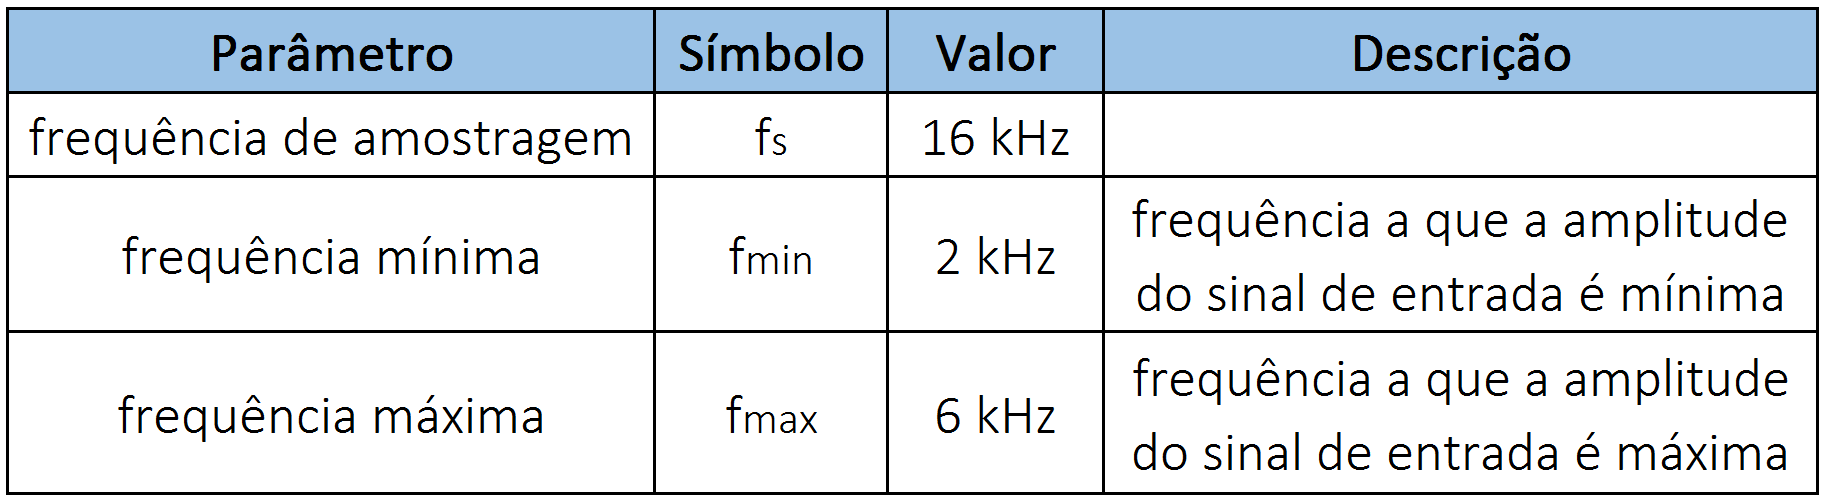
\includegraphics[keepaspectratio=true, scale=0.45]{tabelas/tabela1}
\end{table}

\subsection{} %pergunta 1

Pretende-se primeiramente desenvolver um oscilador de relaxação utilizando uma variável inteira com sinal de 16 \textit{bits} e a circularidade da representação em complemento para dois. Na figura abaixo encontra-se uma representação do sinal a obter.

\begin{figure}[H]
	\centering
	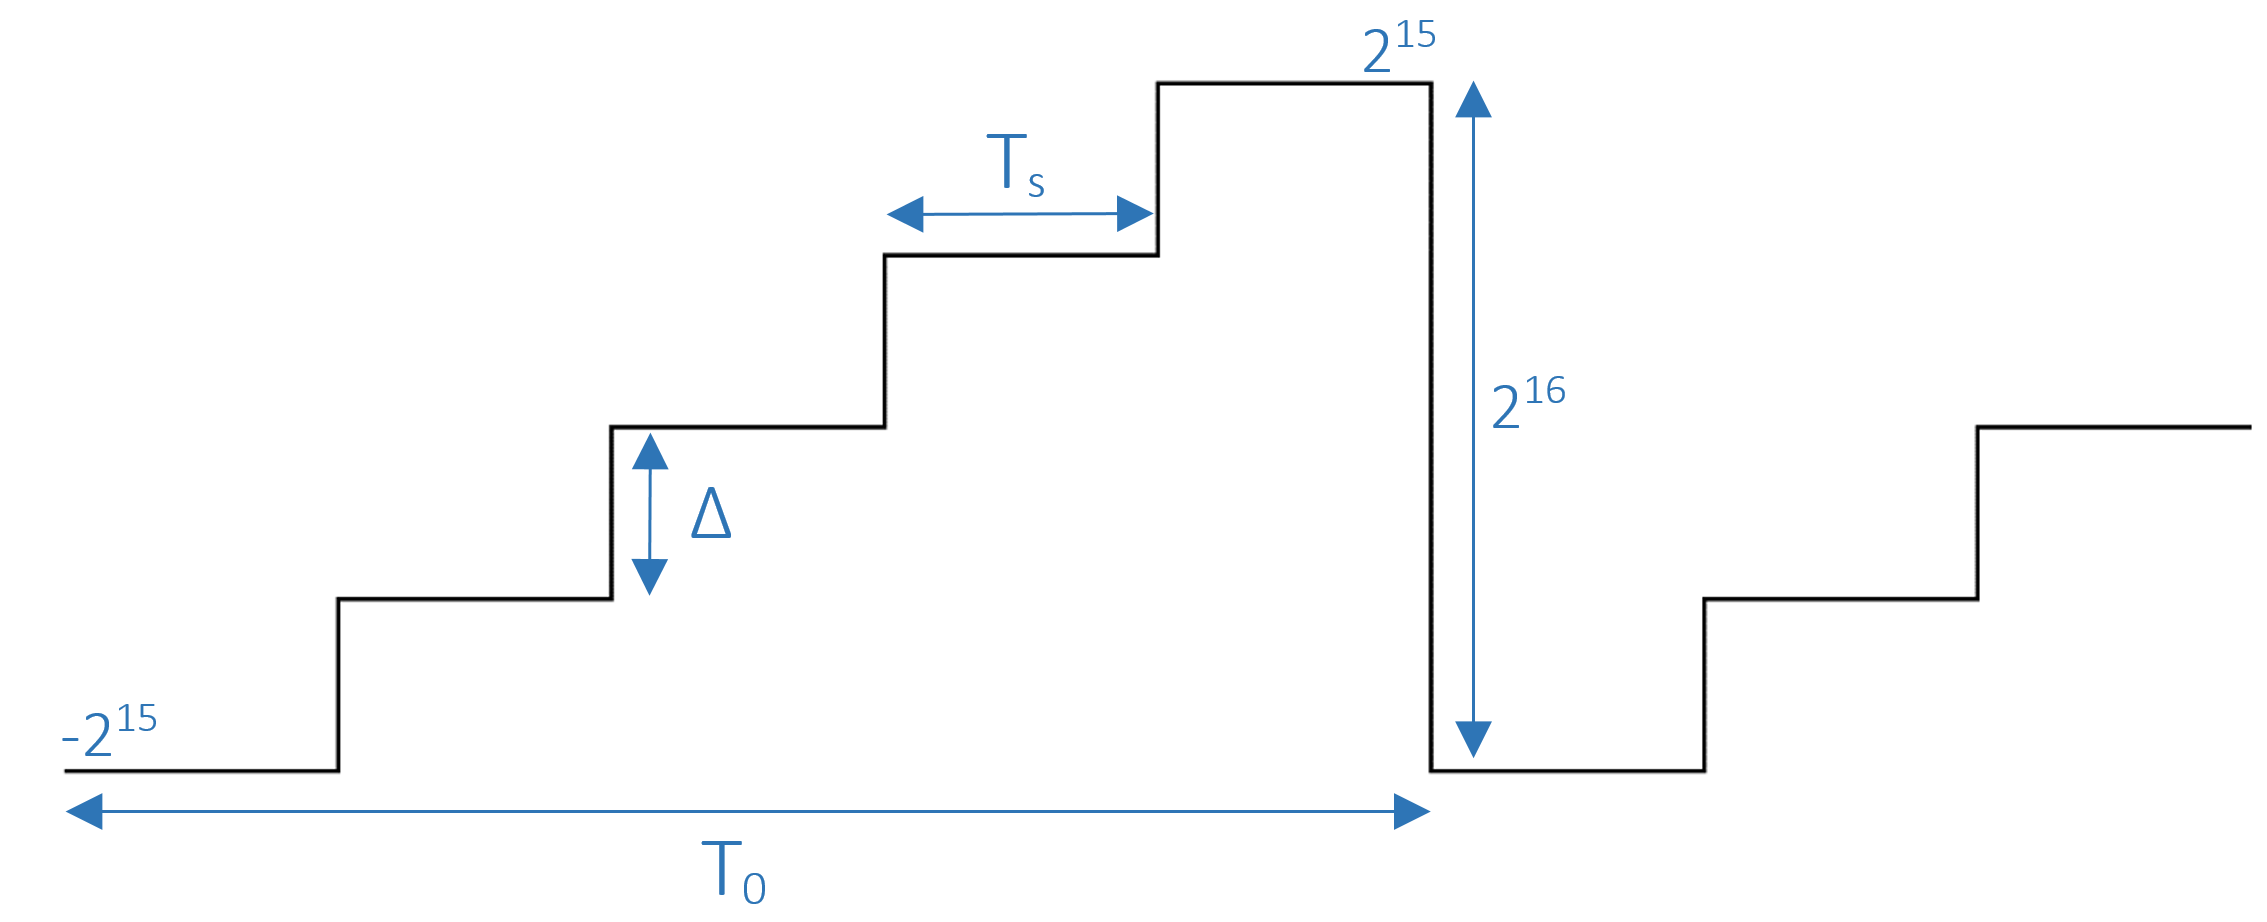
\includegraphics[keepaspectratio=true, scale=0.37]{teoricas/rampa}
	\caption{Esquema do oscilador de relaxação.}
	\vspace{-0.8em}
\end{figure}

\pagebreak

Com recurso à Figura 1 pode-se deduzir que

\vspace{-3mm}
\begin{equation}
f_{0} = \frac{\bigtriangleup}{2^{16}} \times f_{s} \leftrightarrow \bigtriangleup = \frac{f_{0}}{f_{s}} \times 2^{16}.
\end{equation}

Existe uma variável de estado da rampa que a cada $T_{s}$, período de amostragem, é incrementada de $\bigtriangleup$, como se pode ver na Figura 1. A variável de estado da rampa é de 16 \textit{bits} com representação em $Q_{15}$ e, sabendo que o maior número positivo que se pode representar em $Q_{15}$ é $2^{15} - 1 = 32767$ e o menor número negativo que se pode representar é  $-(2^{15} - 1) = -32767$, a variável de estado começa com o valor -32767 e vai até um máximo de 32767. Quando é atingido o valor máximo, 32767, entra em efeito a circularidade da representação em complemento para dois e, assim, a variável de estado não atinge o valor de $2^{15}$, ``dando a volta'' para -32767. 

Relativamente à variável $\bigtriangleup$ esta encontra-se também representada em $Q_{15}$. O NCO tem como característica uma frequência $f_{0}$ que varia entre 2 kHz e 6 kHz. Estes valores são controlados a partir da amplitude do sinal de entrada. Quando esta for minima, a frequência $f_{0}$ é de 2 kHz e quando for máxima, a frequência $f_{0}$ é de 6 kHz. Com estas especificações pode-se calcular três valores de $\bigtriangleup$ com recurso à equação (2.1), para a frequência mínima, a frequência média e a frequência máxima.

\begin{table}[H]
	\centering
	\caption{Valores de $\bigtriangleup$ para as três frequências especificadas.}
	\vspace{-1.5mm}
	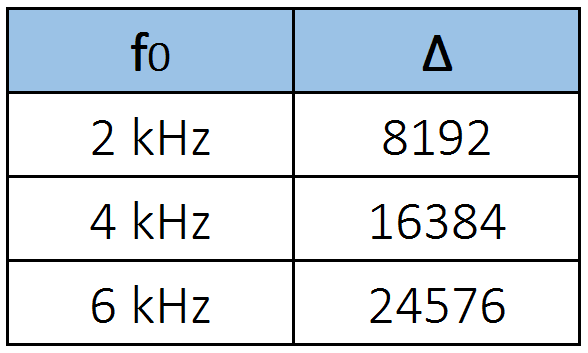
\includegraphics[keepaspectratio=true, scale=0.45]{tabelas/tabela2}
\end{table}

Em código, a variável de estado da rampa é \texttt{status} e a variável que representa os incrementos é \texttt{delta}. No código abaixo está a criação da rampa para um frequência de 4 kHz.

\begin{lstlisting}[language=C]
void main(){

	short delta = 16384;
	short status = -32767;

	while(1){
		...	
		//criacao da rampa	
		status = status + delta;
		...
	}
}
\end{lstlisting}

Nas figuras da próxima página pode-se ver o sinal obtido experimentalmente que representa a rampa para dois valores diferentes de frequência $f_{0}$.

\begin{figure}[H]
	\centering
	\subfloat[]{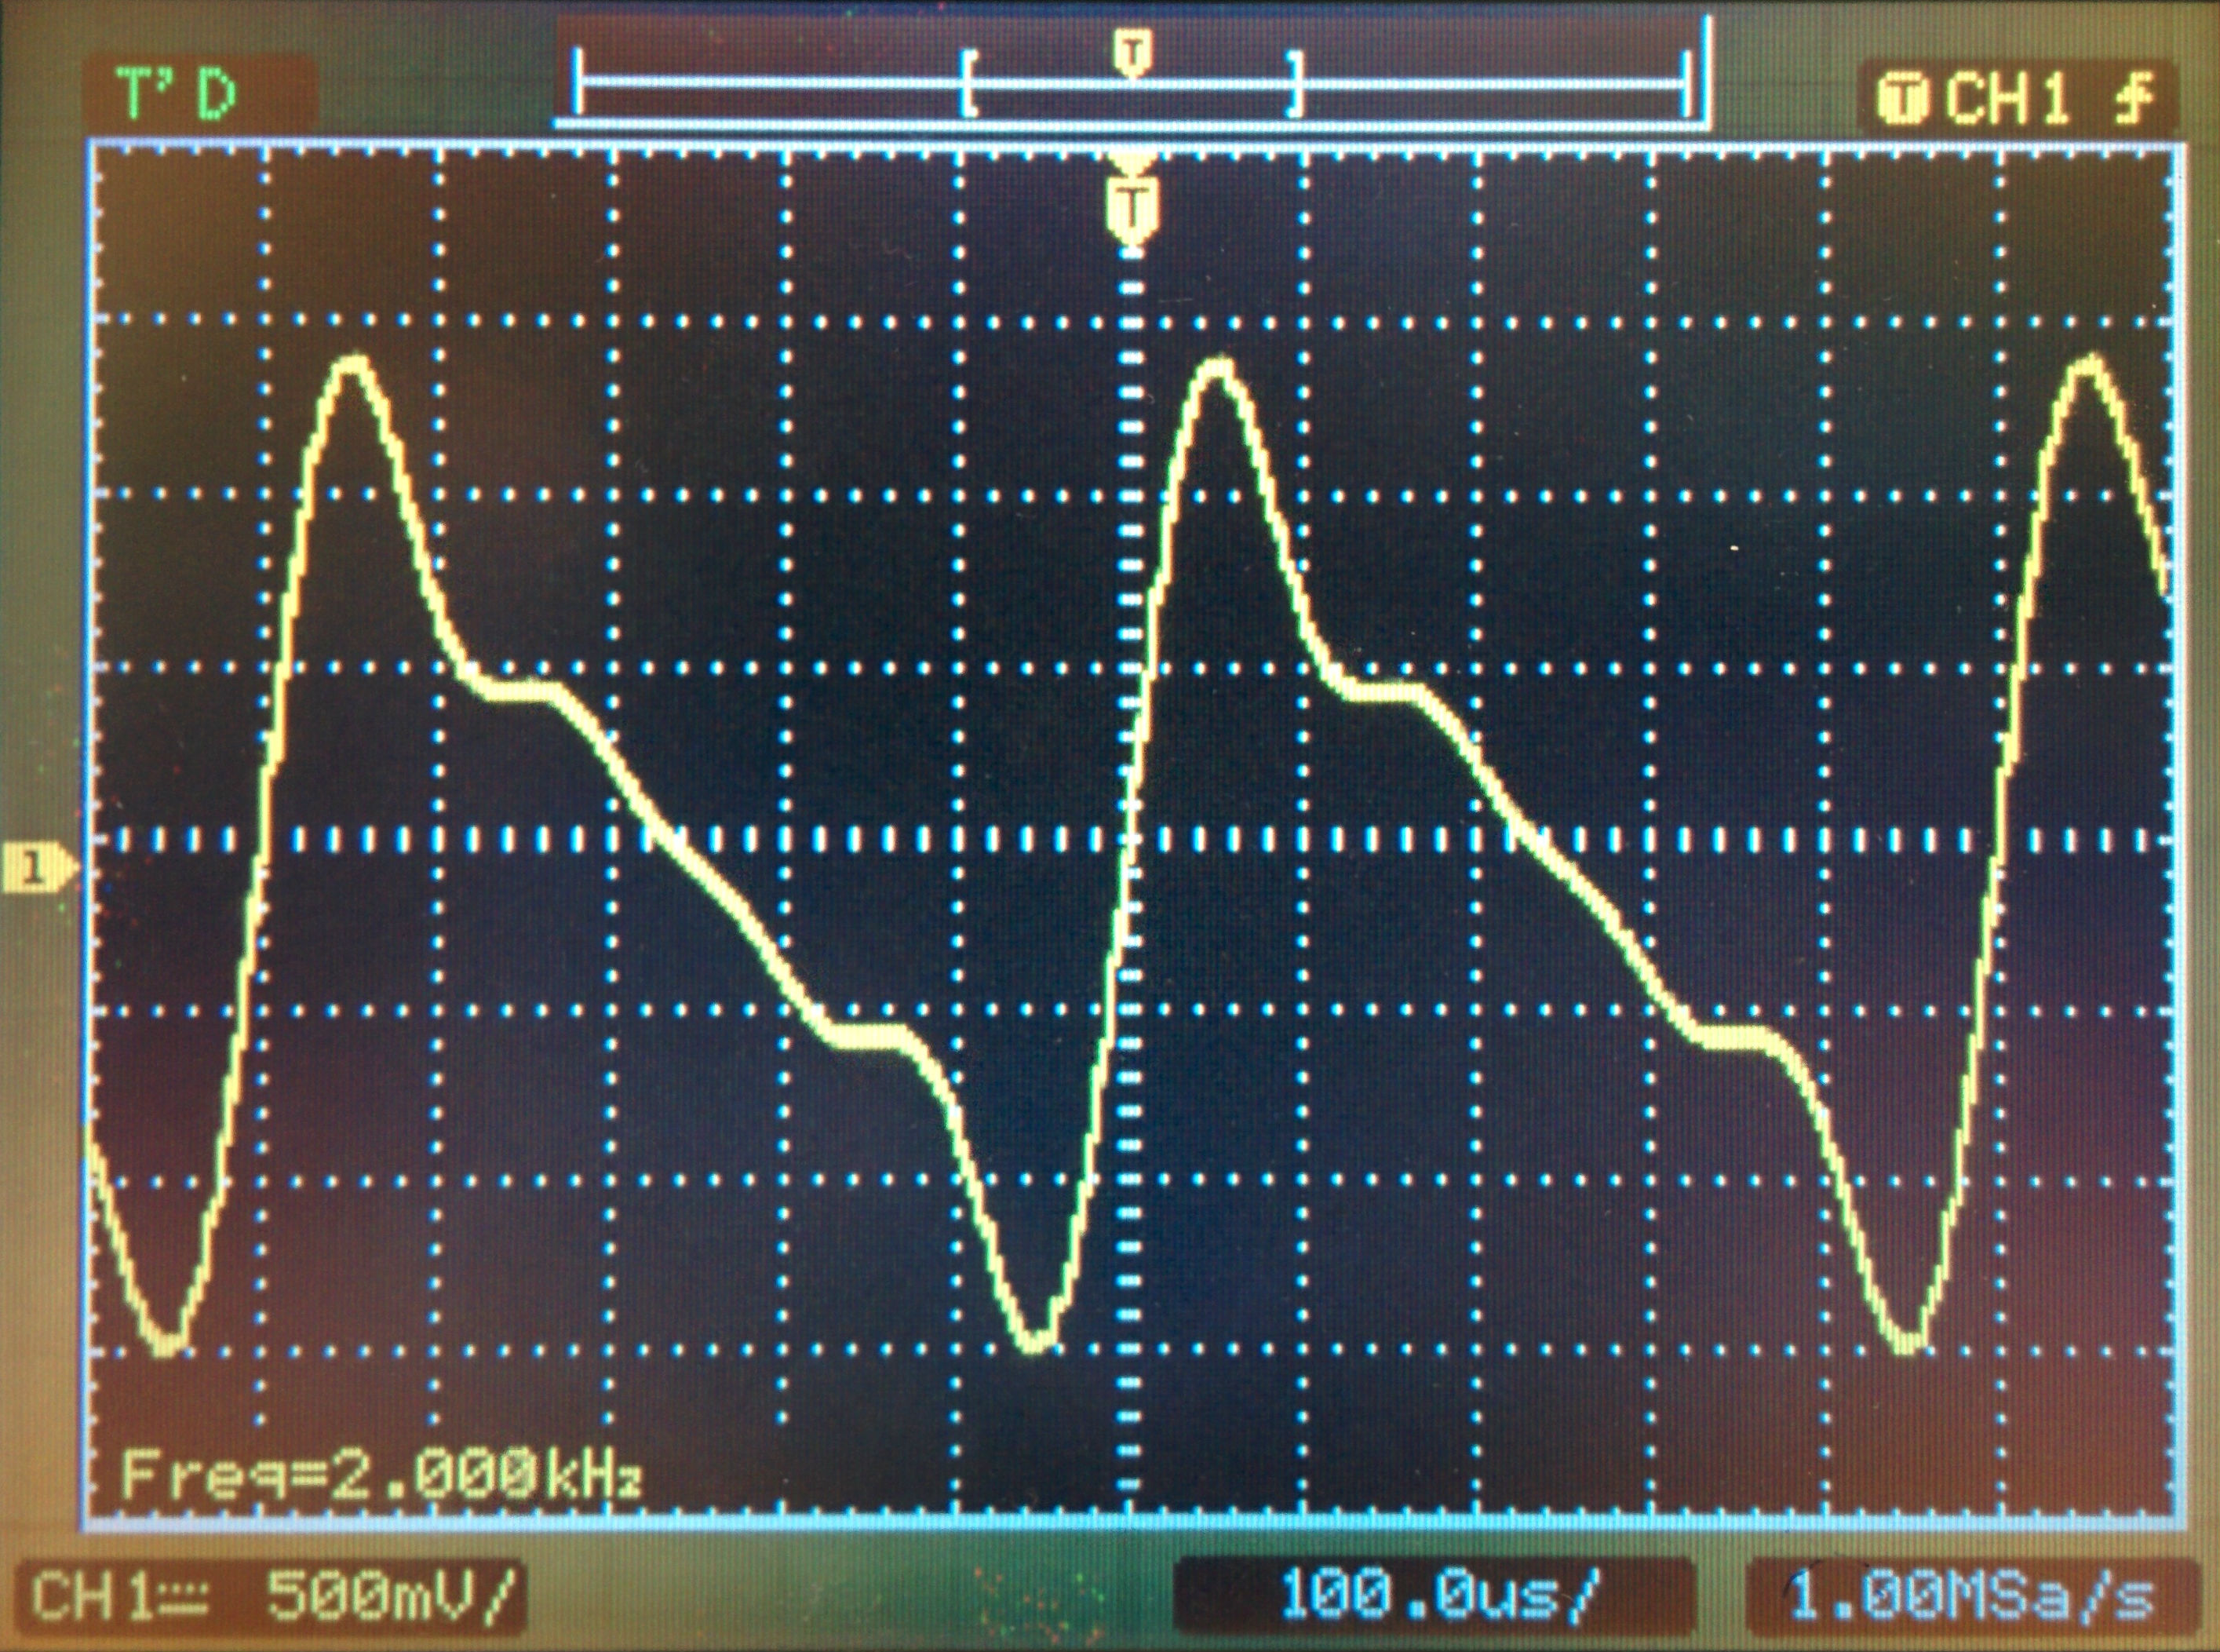
\includegraphics[keepaspectratio=true, scale=0.073]{exps/rampa2K}}
	\hspace{8mm}
	\subfloat[]{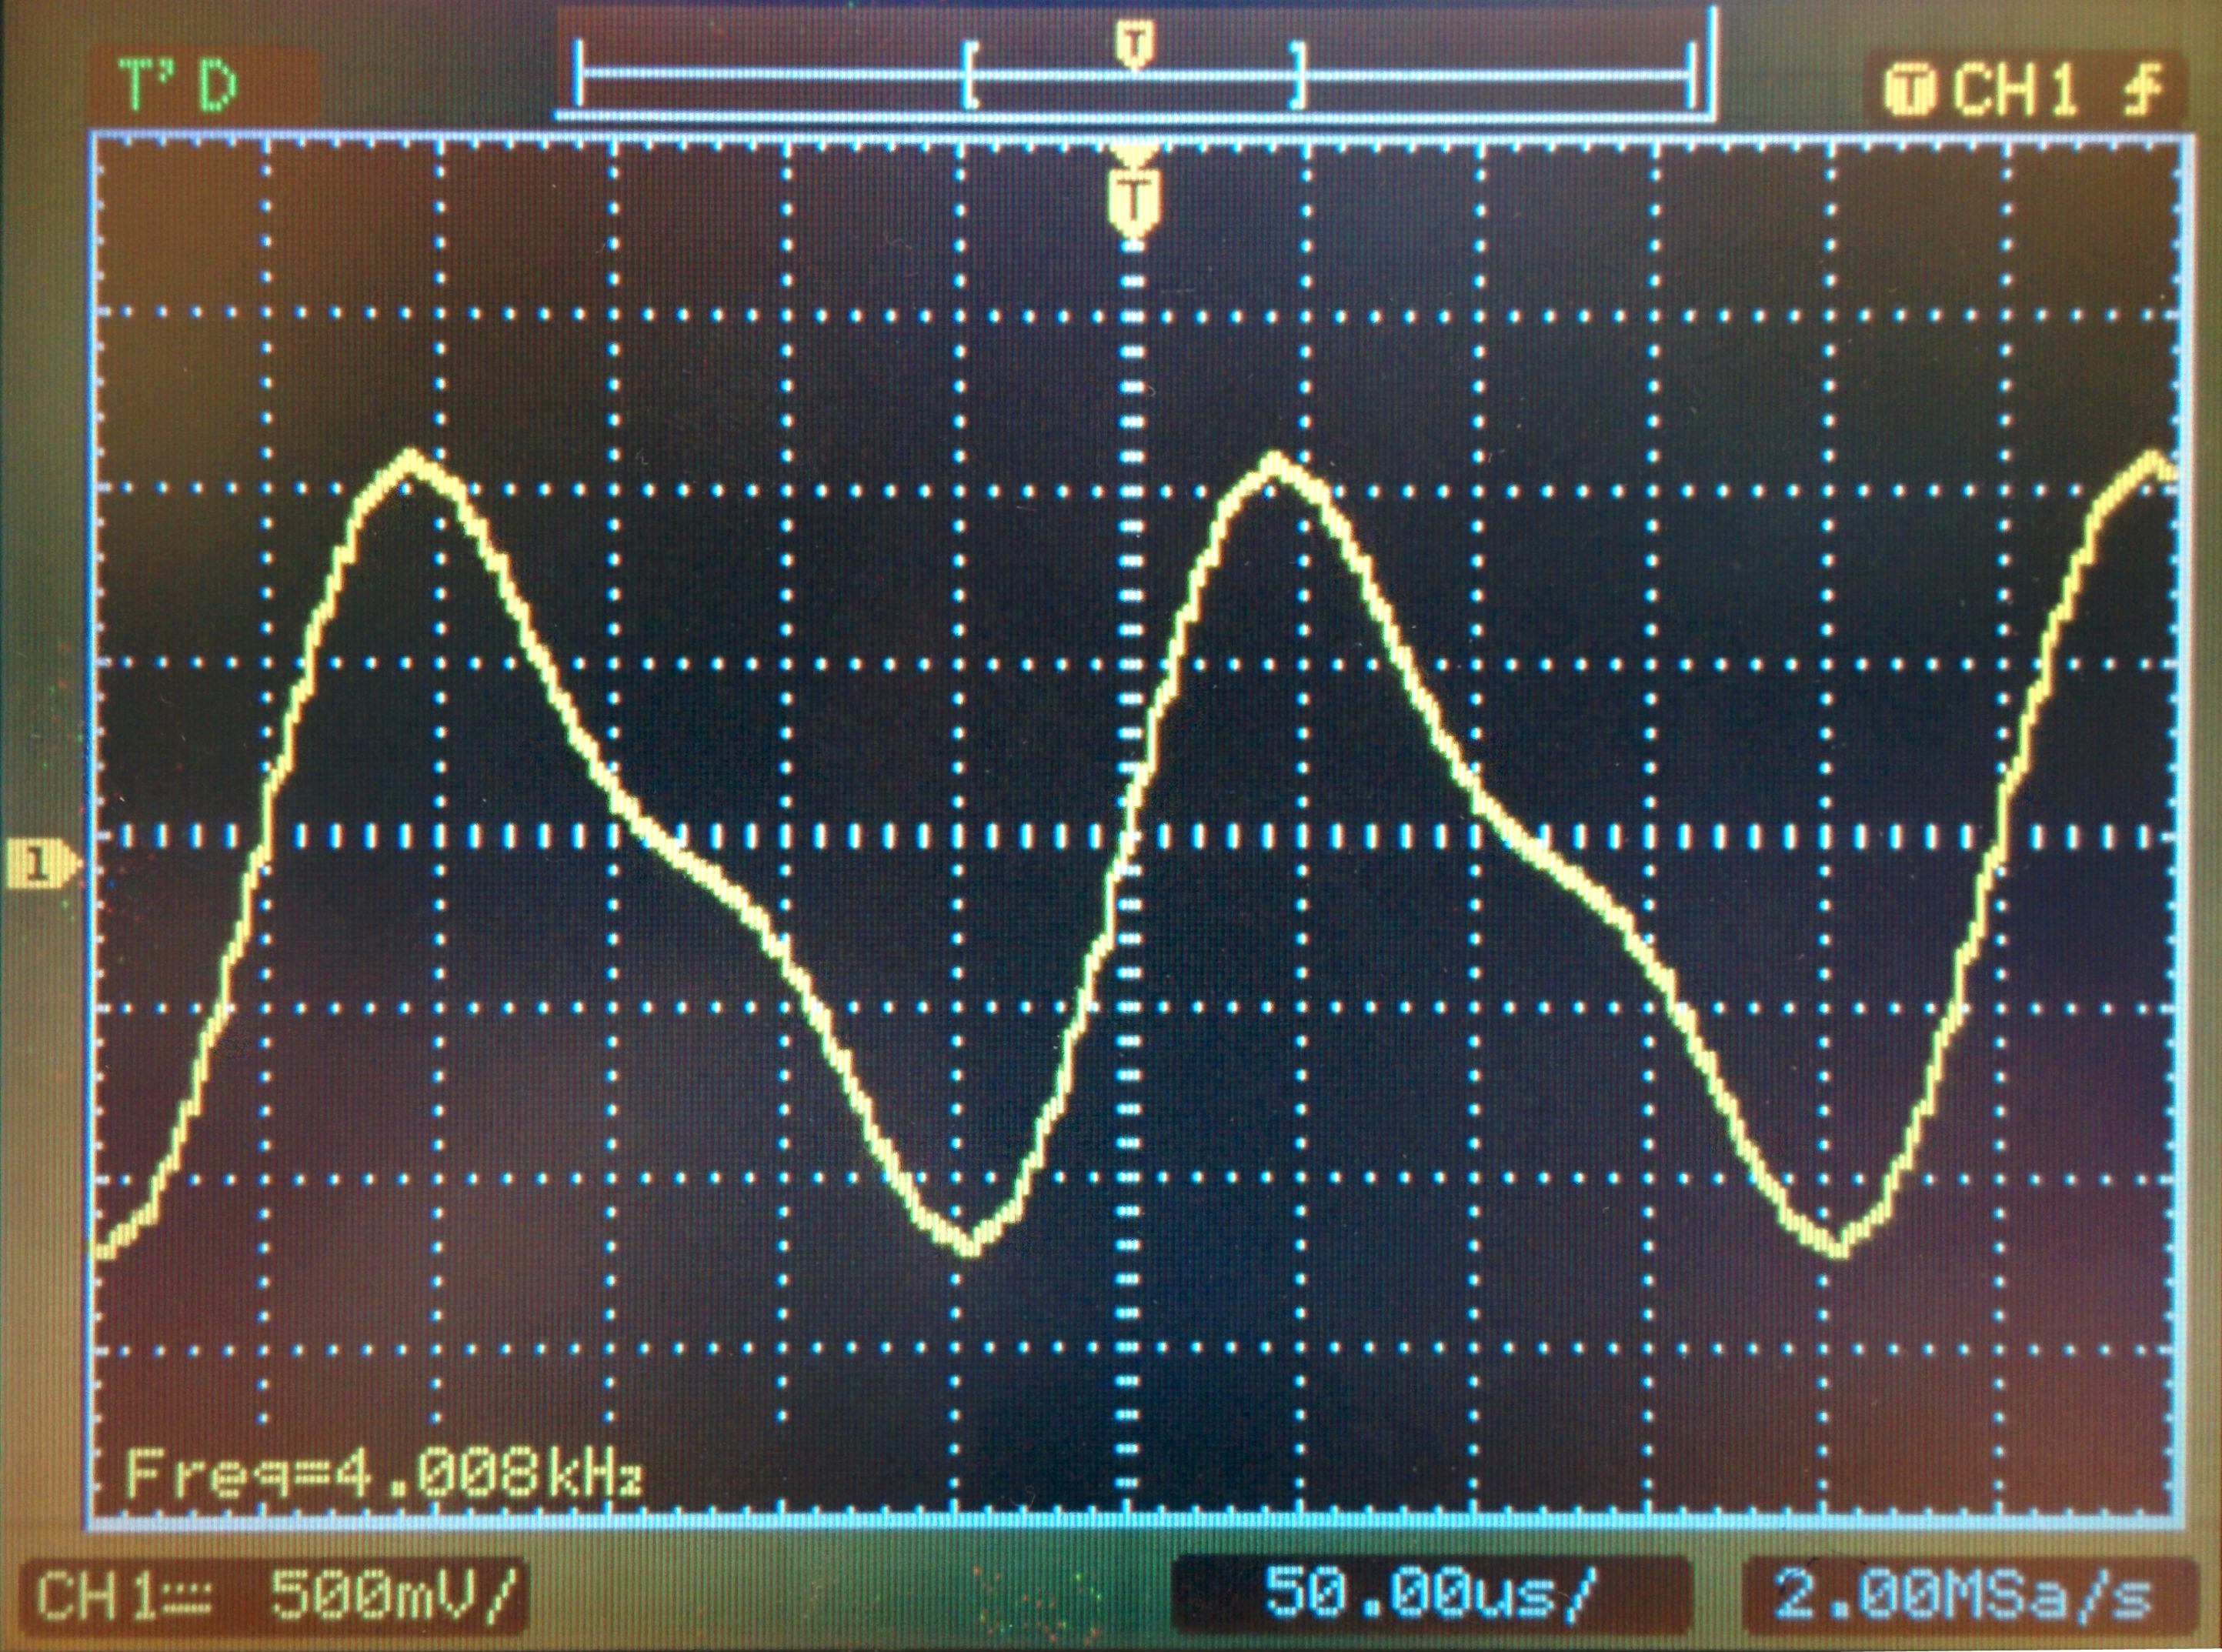
\includegraphics[keepaspectratio=true, scale=0.0719]{exps/rampa4K}}
	\linebreak
	\subfloat[]{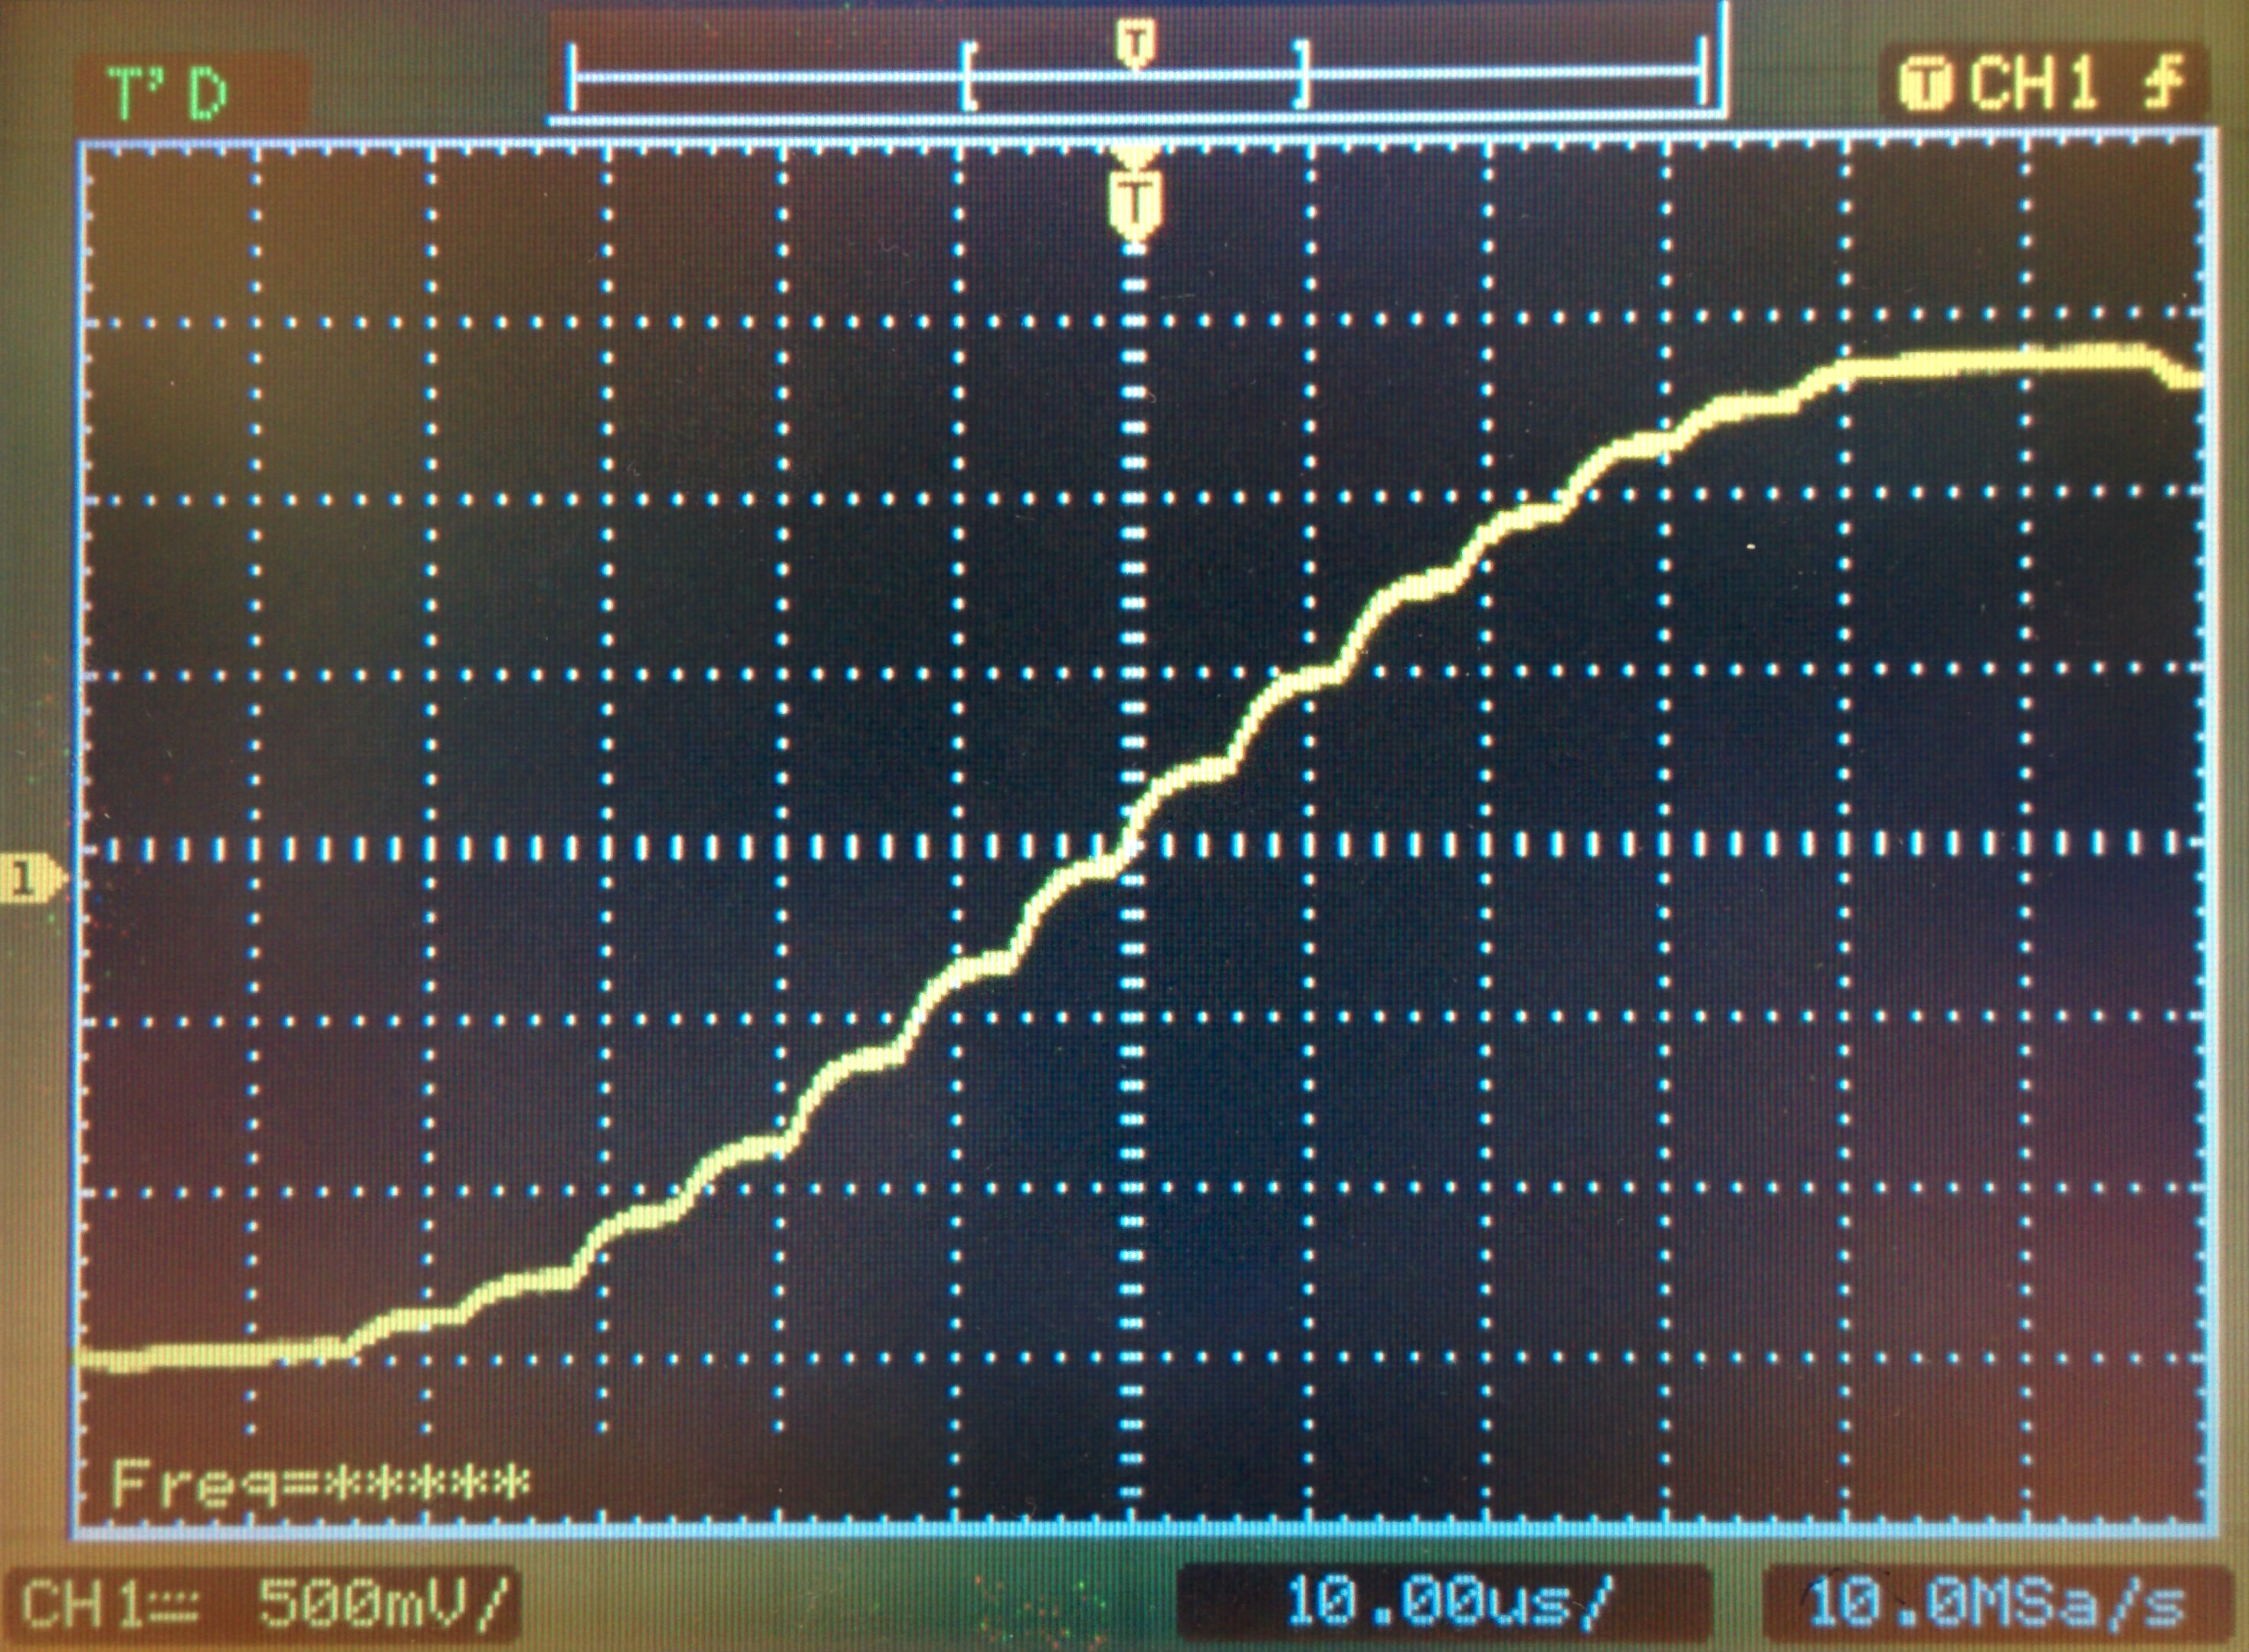
\includegraphics[keepaspectratio=true, scale=0.073]{exps/zoomrampa}}
	\vspace{-0.8em}
	\caption{Oscilador de relaxação para $f_{0}$ = 2 kHz (a), oscilador de relaxação para $f_{0}$ = 4 kHz (b) e pormenor da rampa criada (c).}
	\vspace{-0.8em}
\end{figure}

Como se pode ver na Figura 2(c), por comparação com o esperado teoricamente da Figura 1, o oscilador de relaxação implementado funciona de acordo com o previsto.

\subsection{} %pergunta 2

De forma a criar a \textit{look-up-table} (LUT) com 32 valores positivos de meio período da função seno, é necessário começar por determinar esses valores, para que, posteriormente, os mesmos sejam convertidos para o formato mais preciso de representação, $Q_{15}$, uma vez que se encontram no intervalo [-1, 1]. Assim, tendo em conta que meio período da função seno é $\pi$, podemos calcular os valores da seguinte maneira:

\vspace{-3mm}
\begin{equation}
a_{k} = \sin \left( \frac{\pi}{32}k \right), k = 0, 1, \ldots, 32.
\end{equation}

Os 32 valores determinados são então convertidos para o formato $Q_{15}$, recorrendo a:

\vspace{-3mm}
\begin{equation}
a_{k_{15}} = \text{round}\left(a_{k} \times 2^{15} \right),
\end{equation} 

sendo assim criada a LUT pretendida.

Apresenta-se de seguida o excerto de código onde é declarada a LUT com os valores de meio período da função seno, no vector \texttt{sine} que tem 33 posições, cada uma de 16 \textit{bits}. \todo{se calhar explicar porquê 33 valores e nao os 32 pedidos - david}

\begin{lstlisting}[language=C]
	...
		//LUT do seno
		short sine[33] = {0,3212,6393,9512,12540,15447,18205,20788,23170,25330,27246,28899,30274,31357,		32138,32610,32767,32610,32138,31357,30274,28899,27246,25330,23170,20788,18205,	15447,12540,9512,6393,3212,0}; 
	...
\end{lstlisting}

\subsection{} %pergunta 3

Para que se possa aceder aos valores da função seno, é utilizada a variável de estado do oscilador, \texttt{status}, como índice da LUT. Apenas 5 \textit{bits} da variável são utilizados para endereçar a LUT, sendo criada a variável \texttt{i}, tal como especificado na Figura 3, onde a variável de estado do oscilador é representada por \texttt{x}.

\begin{figure}[H]
	\centering
	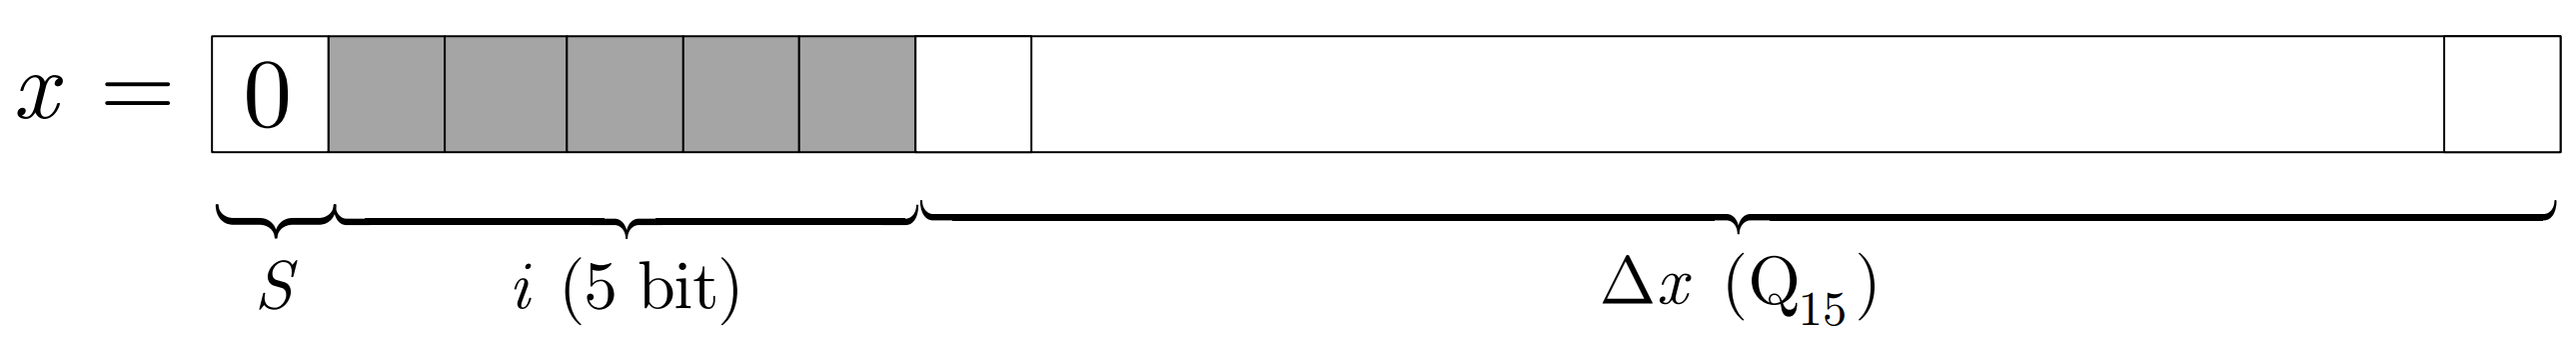
\includegraphics[keepaspectratio=true, scale=0.27]{teoricas/seno}
	\caption{Representação da variável do estado do oscilador.}
	\vspace{-0.8em}
	\label{fig:variavelestado}
\end{figure}

De modo a aceder aos 5 \textit{bits} pretendidos da variável de estado, é realizado um deslocamento de 10 \textit{bits} para a direita, sendo, de seguida, utilizada a função lógica \texttt{AND} com a máscara \texttt{31} (5 \textit{bits} menos significativos com o valor lógico \texttt{1}). É apresentado o excerto de código que realiza o procedimento especificado. 

\begin{lstlisting}[language=C]
	...
		//indexar a LUT e obter os valores do seno
		i = status >> 10;
		i = i & 31;
		y1 = sine[i]; 
	...
\end{lstlisting}

\subsection*{2.4 e 2.5} %perguntas 4 e 5

Foram criadas duas variáveis com o objectivo de controlar a amplitude e frequência do sinal sinusoidal. A variável \texttt{delta} representa o controlo da frequência e a variável \texttt{amp} representa o controlo da amplitude. O código que permite implementar este controlo é apresentado de seguida.  

\begin{lstlisting}[language=C]
void main(){
	...
	//variavel de controlo de frequencia
	short delta = 0
	//variavel de controlo da amplitude: define um ganho de 1/2 
	short amp = 16384; 
	short yf = 0;
	...
	while(1){          
		if(intflag != FALSE){
		...	
		//obtencao do valor para a frequencia		
		delta = 16384 + (inbuf>>2); 
		 ...
		//controlo da amplitude e frequencia
		yf = (y1*delta<<1)>>16);
		y = (yf*amp<<1)>>16);
		
		if(status < 0)
			y = -y;
			
		AIC_buffer.channel[LEFT] = y;
		}
	}
}
\end{lstlisting}

Analisando a Tabela 2 verifica-se que o valor de \texttt{delta} oscila com uma amplitude de 8192 em torno de 16384, $\bigtriangleup_{0}$ . Ou seja, $f_{0}$ tem uma frequência central em 4 kHz, oscilando com uma amplitude de 2 kHz. O incremento do oscilador é obtido de acordo com a seguinte equação, onde $x$ é a amplitude do sinal de entrada: 

\vspace{-3mm}
\begin{equation}
\bigtriangleup = \bigtriangleup_{0} + kx.
\end{equation}

Com esta conclusão, teve de se garantir que o valor da amplitude do sinal de entrada não ultrapassa 8192, mantendo a relação entre cada amostra. Optou-se por dividir o valor de cada amostra por 4, $k = 1/4$, pois a amplitude máxima é de 32767, o equivalente a um \textit{shift} de 2 \textit{bits} para a direita. 

Em baixo está o código referente ao cálculo para obter o valor de \texttt{delta}, sendo que todas as variáveis definidas neste excerto são de 16 \textit{bits}, \texttt{short}, em formato $Q_{15}$.

\begin{lstlisting}[language=C]
	...	
		//obtencao do valor para a frequencia		
		delta = 16384 + (inbuf>>2); 
	...
\end{lstlisting}

Tendo o valor de \texttt{delta}, é simples obter a amplitude de cada amostra do sinal de saída, multiplicando \texttt{delta} por \texttt{y1}, valor obtido da LUT referente à questão 2.2. Em baixo está representado um excerto do código que demonstra a obtenção da amplitude do sinal de saída. Todas as variáveis são de 16 \textit{bits}, tendo \texttt{y1} e \texttt{delta} o formato de $Q_{15}$, como também \texttt{yf}. Isto deve-se ao facto de o formato do resultado da multiplicação com duas variáveis em $Q_{15}$ ser $Q_{30}$ com replicação do \textit{bit} de sinal. Assim, é necessário efectuar um \textit{shift} para a esquerda para remover o \textit{bit} de sinal replicado, resultando num formato final de $Q_{31}$, para 32 bits. Para se poder armazenar numa variável de 16 \textit{bits}, no formato $Q_{15}$, é necessário efectuar um \textit{shift} de 16 posições para a direita, permitindo armazenar os 16 \textit{bits} mais significativos do resultado de 32 \textit{bits}.

O código apresentado de seguida demonstra a explicação referida.

\begin{lstlisting}[language=C]
	...
		//controlo da amplitude e frequencia
		yf = (y1*delta<<1)>>16);
	...
\end{lstlisting}

Para o controlo da amplitude do sinal de saída, multiplica-se o resultado final obtido anteriormente por uma constante de 16 \textit{bits} em formato $Q_{15}$. Está representado um excerto de código que demonstra a alteração da amplitude do sinal de saída. Neste caso todas as variáveis são também de 16 \textit{bits}, tendo \texttt{yf} e \texttt{amp} o formato de $Q_{15}$, como também \texttt{y}. Para armazenar a variável \texttt{y} em $Q_{15}$ recorre-se à mesma lógica explicada anteriormente de fazer 15 \textit{shifts} para a direita ao resultado da multiplicação.

O código apresentado de seguida demonstra a explicação referida.

\begin{lstlisting}[language=C]
	...
		//controlo da amplitude e frequencia
		y = (y_f*amp<<1)>>16);
	...
\end{lstlisting}

\subsection*{2.6} %pergunta 6

\todo{teddy}

\subsection*{2.7} %pergunta 7

Pretende-se agora melhorar a qualidade do oscilador sinusoidal utilizando interpolação linear. Esta interpolação é feita lendo dois valores consecutivos, $y_{1}$ e $y_{2}$, da LUT do seno e depois obter o valor sinusoidal interpolado com recurso à seguinte equação

\vspace{-3mm}
\begin{equation}
y = y_{1} + (y_{2} - y_{1})
\end{equation}

Na Figura \ref{fig:variavelestado}, onde se encontra representada a variável de estado da rampa, pode-se ver que os 10 \textit{bits} menos significativos 

\todo{margarida}

\subsection*{2.8} %pergunta 8

\todo{margarida}

\section{Projecto $\#$2 - Transmissor BPSK}

Neste projecto, pretende-se implementar o codificador de um transmissor BPSK (Binary Phase-shift Keying), representado na Figura X.

\begin{figure}[H]
	\centering
	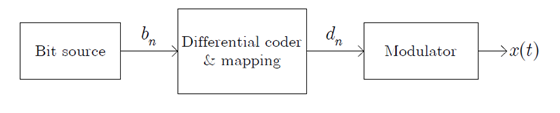
\includegraphics[keepaspectratio=true, scale=1.0]{teoricas/bpsk}
	\caption{Esquema de um transmissor BPSK.}
	\vspace{-0.8em}
\end{figure}


O codificador tem como entrada os bits bn, que se trata de uma sequência que vai alternando entre o valor lógico \texttt{'0'} e o valor lógico \texttt{'1'} ($b_n$ = 1, 0, 1, 0,….) e como saída os valores $d_n$, que podem ser $-1$ ou $+1$. O codificador realiza a operação $c_n = c_{n-1} \oplus b_n$, considerando $c_0$ = ‘0’, para que depois possam ser determinados a sequência dn, de acordo com o mapeamento:

\vspace{-3mm}
\begin{equation}
	c_{n} = \text{'}0\text{'}\to d_{n} = +1;   
\end{equation} 
\begin{equation}
c_{n} = \text{'}1\text{'}\to d_{n} = -1;
\end{equation}

Assim, o sinal modulado BPSK é dado por:

\vspace{-3mm}
\begin{equation}
	s(t) = \sin (2 \pi f_0 t + \pi c_n) = d_n \sin (2 \pi f_0 t) 
\end{equation} 

Ou, usando tempo discreto:

\vspace{-3mm}
\begin{equation}
	s_{n} = s(n T_s) = d_n \sin (2\pi f_0 T_s n)
\end{equation} 

É utilizada uma frequência de amostragem, $f_s=1/T_s$ , de 16 \textit{kHz} e uma frequência da portadora, $f_0$, de 4 \textit{kHz}. A taxa de bits é de $f_b$ = 1\textit{kbps}, por isso por cada bit, há 4 períodos da portadora.  


\subsection{} %pergunta 1

Os bits da sequência $b_n$ são implementados recorrendo a um contador, uma vez que a cada 16 amostras do sinal de entrada, é necessário que haja uma alteração do bit seguinte da sequência $b_n$, passando de \texttt{'0'} para \texttt{'1'} ou vice-versa. Para que seja realizada essa alteração, é utilizada a função XOR do bit $b_n$ anterior com \texttt{'1'}. É assim apresentado o excerto de código que implementa a sequência de bits $b_n$. 

\begin{lstlisting}[language=C]
	...
	if(b_i>15){
		b_i=0;
		b_n=(b_n^1); 
	...
	}
	b_i++; 
\end{lstlisting}

Foi criado outra solução para a obtenção da sequência $b_n$ com objectivo de não utilizar a instrução condicional, \texttt{if}. Seguiu-se o conselho do enunciado de usar um contador que quando ocorre o \textit{overflow} gera um novo \textit{bit} alternado. Está representado de seguida o excerto de código:

\begin{lstlisting}[language=C]
	...
	 b_i++;			
	 b=(b_i&16)>>4; // mascara para obter o bit de overflow
	 b_n=(b_n^b);	// xor para alternar o bit bn
	 b_i=(b_i&15);  // obtencao dos 4 bits menos significativos
	...
\end{lstlisting}

Como se pode observar, a ocorrência de \textit{overflow} acontece quando o contador atinge 16, \texttt{b\_i} (O valor 16 deve-se ao facto que a frequência de amostragem, de 16 \textit{kHz}, ser divida por esse mesmo valor deforma a obter o resultado de 1 \textit{kbps}). Para detectar esta ocorrência aplica-se a máscara 16 (o quinto \textit{bit} menos significativo com o valor lógico 1) e efectua-se um \textit{shift} 4 posições para a direita. De seguida, aplica-se a função XOR com o resultado anterior com a variável \texttt{b\_n} de forma a obter uma sequência $b_n$ que varia alternadamente entre \texttt{'0'} e \texttt{'1'} ou vice-versa a uma taxa de $f_b$ = 1 \textit{kbps}.


Com o \textit{bit-rate}, $b_n$, criado aplica-se o codificador diferencial de forma a gerar o sinal $c_n$, pela seguinte equação:

\vspace{-3mm}
\begin{equation}
		c_n = c_{n-1} \oplus b_n
\end{equation} 

A equação anterior foi implementada no ciclo de criação do \textit{bit-rate}, $b_n$,  Aplicando a função XOR do bit $c_{n-1}$ com $b_n$, de seguida mostra-se o código;
\begin{lstlisting}[language=C]
	c_n = 0;
	...
	if(b_i>15){
		b_i=0;
		b_n=(b_n^1);
		c_n=c_n^b_n; //codificador diferencial
		...
	}
	b_i++;
	...
\end{lstlisting}



		
\subsection{} %pergunta 2



\subsection{} %pergunta 3

\todo{margarida}

\section{Conclusões}

\end{document}